% 2014 全国卷Ⅰ理科第 19 题：三棱柱；短虚线为经过隐藏顶点 C 的棱。
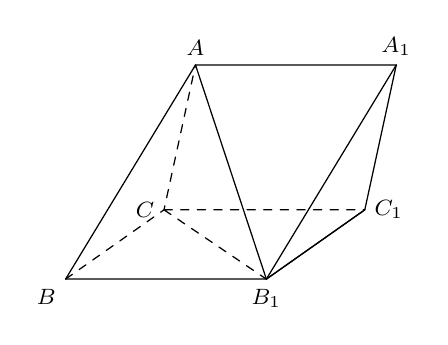
\begin{tikzpicture}[font=\footnotesize,line width=.45pt,line cap=round,line join=round]
  \coordinate (B) at (0,0); \coordinate (B1) at (2.55,0); \coordinate (C) at (1.25,.88); \coordinate (C1) at (3.80,.88);
  \coordinate (A) at (1.65,2.72); \coordinate (A1) at (4.20,2.72);
  \draw (B)--(A)--(A1)--(B1)--cycle; \draw (A1)--(C1)--(B1); \draw (A)--(B1); \draw (B1)--(C1);
  \draw[dashed] (B)--(C)--(A) (C)--(C1) (C)--(B1);
  \node[below left] at (B) {$B$}; \node[below] at (B1) {$B_1$}; \node[left] at (C) {$C$}; \node[right] at (C1) {$C_1$};
  \node[above] at (A) {$A$}; \node[above] at (A1) {$A_1$};
\end{tikzpicture}
